\documentclass[0-thesis.tex]{subfiles}

\begin{document}
The previous chapter introduced the update architecture proposed by the thesis and the
design of a prototype aimed to evaluate it. This chapter will analyze the proposed
architecture qualitatively from the SUIT specification as well as quantitatively evaluate
the prototype, measuring energy consumption, communication overhead, and code size.

\section{Qualitative Evaluation of Update Architecture}
\label{sec:qual-evaluation}
The proposed architecture was evaluated in two parts analogous to how the SUIT working
group presented their work, namely architecture and information model. Using the
requirements of each document, a qualitative evaluation of the proposed architecture was
performed. The requirements are gathered from \parencite{suit-architecture,
suit-information-model}.

\subsection{Architecture}
\label{ssec:arch-evaluation}
The SUIT architecture document specified ten requirements a suitable update architecture
should fulfill. Table~\ref{tab:architecture-evaluation} enumerates these with their
corresponding motivations from the viewpoint of the proposed architecture.

\begin{longtable}[]{@{}ll@{}}
    \caption{The SUIT architecture requirements and their motivations.}
    \label{tab:architecture-evaluation}\\
    \toprule
    \begin{minipage}[b]{0.41\columnwidth}\raggedright\strut
    Requirement\strut
    \end{minipage} & \begin{minipage}[b]{0.53\columnwidth}\raggedright\strut
    Motivation\strut
    \end{minipage}\tabularnewline
    \midrule
    \endfirsthead
    \toprule
    \begin{minipage}[b]{0.41\columnwidth}\raggedright\strut
    Requirement\strut
    \end{minipage} & \begin{minipage}[b]{0.53\columnwidth}\raggedright\strut
    Motivation\strut
    \end{minipage}\tabularnewline
    \midrule
    \endhead
    \toprule
    \begin{minipage}[b]{0.41\columnwidth}\raggedright\strut
    Requirement\strut
    \end{minipage} & \begin{minipage}[b]{0.53\columnwidth}\raggedright\strut
    Motivation\strut
    \end{minipage}\tabularnewline
    \midrule
    \endhead
    \toprule
    \begin{minipage}[b]{0.41\columnwidth}\raggedright\strut
    Requirement\strut
    \end{minipage} & \begin{minipage}[b]{0.53\columnwidth}\raggedright\strut
    Motivation\strut
    \end{minipage}\tabularnewline
    \midrule
    \endhead

    \begin{minipage}[t]{0.41\columnwidth}\raggedright\strut
    Agnostic to how firmware images are distributed\strut
    \end{minipage} & \begin{minipage}[t]{0.53\columnwidth}\raggedright\strut
    No parts of the architecture assumes a specific suite of protocols or
    algorithms to ensure secure delivery of updates. The architecture does
    specify the usage of technologies such as certificates, asymmetric
    encryption, and authorization tokens, but these elements can be
    implemented in a wide variety of ways using different protocols,
    algorithms, and certificate/token types. The profiles provided in the
    thesis are examples of how specific incarnations of the architecture
    could look like.\strut
    \end{minipage}\tabularnewline
    \begin{minipage}[t]{0.41\columnwidth}\raggedright\strut
    Friendly to broadcast delivery\strut
    \end{minipage} & \begin{minipage}[t]{0.53\columnwidth}\raggedright\strut
    The architecture itself does not limit broadcast delivery and through
    correct usage of the manifest broadcasted updates will not be
    incorrectly installed by devices other than the intended recipients.
    Choice of technology can limit the usage of broadcasting, such as DTLS,
    but this is implementation specific.\strut
    \end{minipage}\tabularnewline
    \begin{minipage}[t]{0.41\columnwidth}\raggedright\strut
    Use state-of-the-art security mechanisms\strut
    \end{minipage} & \begin{minipage}[t]{0.53\columnwidth}\raggedright\strut
    The architecture is based on asymmetric cryptography using certificates
    as well as access authorization through whitelists and possibly tokens
    for fine-grain authorization. Choice of key algorithms and token types
    will affect the cryptographic strength of the system, allowing for both
    smaller and less strong keys and tokens or larger and strong keys and
    tokens.\strut
    \end{minipage}\tabularnewline
    \begin{minipage}[t]{0.41\columnwidth}\raggedright\strut
    Rollback attacks must be prevented\strut
    \end{minipage} & \begin{minipage}[t]{0.53\columnwidth}\raggedright\strut
    By specifying a monotonically increasing sequence number in the
    manifest, devices can make sure they are installing fresh images.
    Manifests are signed through COSE which ensures authenticity, an
    assailant would not be able to modify a manifest and then recompute a
    valid signature.\strut
    \end{minipage}\tabularnewline
    \begin{minipage}[t]{0.41\columnwidth}\raggedright\strut
    High reliability\strut
    \end{minipage} & \begin{minipage}[t]{0.53\columnwidth}\raggedright\strut
    This is an implementation specific requirement, however the storage
    element of the manifest aids in achieving safe storage of a new image.
    After a successful update, devices are to re-register at servers. No
    acknowledgment means the server knows the update still must be applied,
    thus an interrupted update can be redistributed.\strut
    \end{minipage}\tabularnewline
    \begin{minipage}[t]{0.41\columnwidth}\raggedright\strut
    Operate with a small bootloader\strut
    \end{minipage} & \begin{minipage}[t]{0.53\columnwidth}\raggedright\strut
    The thesis suggests to store an unencrypted image alongside its digest
    for the bootloader to be minimal, only needing support for calculating a
    SHA256 digest of the image at boot. All information about whether or not
    to perform the update is encoded in conditions in the manifest, and can
    be stored with small memory usage.\strut
    \end{minipage}\tabularnewline
    \begin{minipage}[t]{0.41\columnwidth}\raggedright\strut
    Small parsers\strut
    \end{minipage} & \begin{minipage}[t]{0.53\columnwidth}\raggedright\strut
    The manifest format used in the thesis is simple, complete, and
    extensible. Parsing it requires storing the key/value pairs in
    predefined structures which is doable even with a very small
    parser.\strut
    \end{minipage}\tabularnewline
    \begin{minipage}[t]{0.41\columnwidth}\raggedright\strut
    Minimal impact on existing firmware formats\strut
    \end{minipage} & \begin{minipage}[t]{0.53\columnwidth}\raggedright\strut
    The architecture makes no assumptions about firmware formats. It is up
    to the implementer to ensure the images are prepared for updating and
    that the bootloader contains the necessary functionality. Transporting
    the images is the same regardless of content.\strut
    \end{minipage}\tabularnewline
    \begin{minipage}[t]{0.41\columnwidth}\raggedright\strut
    Robust permissions\strut
    \end{minipage} & \begin{minipage}[t]{0.53\columnwidth}\raggedright\strut
    The architecture is based on asymmetric cryptography using certificates
    for identity and confidentiality, and whitelists of servers and
    operators as possibly tokens for authorization. Different deployments
    have different security and performance requirements, the architecture
    is flexible by allowing different kinds of key algorithms, encryption
    schemes, and token types. Some deployments may not need tokens at all as
    authentication is done on a device level and whitelists are sufficient,
    white other deployments wanting to update specific pieces of a device
    may need fine-grained authorization through tokens. Different devices in
    the same deployment can have different authorization configurations, for
    instance by accepting different types of tokens.\strut
    \end{minipage}\tabularnewline
    \begin{minipage}[t]{0.41\columnwidth}\raggedright\strut
    Operating modes\strut
    \end{minipage} & \begin{minipage}[t]{0.53\columnwidth}\raggedright\strut
    The architecture supports the device initiated pull model as well as the
    operator initiated push model. The update server acts as a mediator
    between device and operator as well as a repository for images and
    device profiles, letting the operator query the server for device
    statuses and devices query for updates depending on the model
    used.\strut
    \end{minipage}\tabularnewline
    \bottomrule
\end{longtable}
  
\subsection{Information Model}
\label{ssec:information-evaluation}
The information model had more requirements posed upon it than the architecture and its
implementation forms an important basis for carrying out safe updates.
Table~\ref{tab:information-evaluation} lists the requirements for the information model
alongside their motivations.

\begin{longtable}[]{@{}ll@{}}
    \caption{The SUIT requirements on the information model and their motivations.}
    \label{tab:information-evaluation}\\
    \toprule
    \begin{minipage}[b]{0.41\columnwidth}\raggedright\strut
    Requirement\strut
    \end{minipage} & \begin{minipage}[b]{0.53\columnwidth}\raggedright\strut
    Motivation\strut
    \end{minipage}\tabularnewline
    \midrule
    \endfirsthead
    \toprule
    \begin{minipage}[b]{0.41\columnwidth}\raggedright\strut
    Requirement\strut
    \end{minipage} & \begin{minipage}[b]{0.53\columnwidth}\raggedright\strut
    Motivation\strut
    \end{minipage}\tabularnewline
    \midrule
    \endhead
    \toprule
    \begin{minipage}[b]{0.41\columnwidth}\raggedright\strut
    Requirement\strut
    \end{minipage} & \begin{minipage}[b]{0.53\columnwidth}\raggedright\strut
    Motivation\strut
    \end{minipage}\tabularnewline
    \midrule
    \endhead
    \toprule
    \begin{minipage}[b]{0.41\columnwidth}\raggedright\strut
    Requirement\strut
    \end{minipage} & \begin{minipage}[b]{0.53\columnwidth}\raggedright\strut
    Motivation\strut
    \end{minipage}\tabularnewline
    \midrule
    \endhead

    \begin{minipage}[t]{0.41\columnwidth}\raggedright\strut Installation
    instructions\strut \end{minipage} &
    \begin{minipage}[t]{0.53\columnwidth}\raggedright\strut Installation instructions or
    any sort of directive is not included in the base manifest structure but can be
    implemented in the options field. Directives, shown as an option in
    Figure~\ref{fig:manifest-format}, could be used to indicate decompression algorithms,
    preparation of bootloader etc while other more specific instructions can be
    implemented either as a directive or a new kind of option element specific to that
    deployment.\strut \end{minipage}\tabularnewline
    \begin{minipage}[t]{0.41\columnwidth}\raggedright\strut
    Override non-critical manifest elements\strut
    \end{minipage} & \begin{minipage}[t]{0.53\columnwidth}\raggedright\strut
    The proposed manifest format has the critical elements as a baseline and
    the rest severed into the options field. Defining new option types
    allows for new elements in the manifest, but the devices need to be
    updated for their parsers and manifest checkers to be aware of the new
    elements.\strut
    \end{minipage}\tabularnewline
    \begin{minipage}[t]{0.41\columnwidth}\raggedright\strut
    Modular update\strut
    \end{minipage} & \begin{minipage}[t]{0.53\columnwidth}\raggedright\strut
    Supported through precursor images, dependencies, URI aliases, and the
    use of authorization tokens for more granular updates. For devices with
    several MCUs and applications, possibly several operating systems,
    update access can be controlled through authorization tokens such that a
    vendor can only update their respective part.\strut
    \end{minipage}\tabularnewline
    \begin{minipage}[t]{0.41\columnwidth}\raggedright\strut
    Multiple authorizations\strut
    \end{minipage} & \begin{minipage}[t]{0.53\columnwidth}\raggedright\strut
    Enforced via operator and update server whitelists and authorization
    tokens.\strut
    \end{minipage}\tabularnewline
    \begin{minipage}[t]{0.41\columnwidth}\raggedright\strut
    Multiple payload formats\strut
    \end{minipage} & \begin{minipage}[t]{0.53\columnwidth}\raggedright\strut
    The architecture and manifest format does not make assumptions about the
    payload formats. The mappings of formats to keys in the manifest is
    deployment specific and whatever formats a deployment might opt to use
    can be represented in the manifest together with a SHA256 digest of said
    format.\strut
    \end{minipage}\tabularnewline
    \begin{minipage}[t]{0.41\columnwidth}\raggedright\strut
    Prevent confidential information disclosure\strut
    \end{minipage} & \begin{minipage}[t]{0.53\columnwidth}\raggedright\strut
    The architecture is based on state-of-the-art security mechanisms and
    achieves confidentiality through asymmetric cryptography. Both manifest
    and payload are encrypted and then signed using COSE.\strut
    \end{minipage}\tabularnewline
    \begin{minipage}[t]{0.41\columnwidth}\raggedright\strut
    Prevent devices from unpacking unknown formats\strut
    \end{minipage} & \begin{minipage}[t]{0.53\columnwidth}\raggedright\strut
    Supported through the use of the manifest format element, preconditions,
    overridable/custom directives, and letting the update server decide if
    there is a suitable update for a device by matching against its
    registered profile.\strut
    \end{minipage}\tabularnewline
    \begin{minipage}[t]{0.41\columnwidth}\raggedright\strut
    Specify version numbers of target firmware\strut
    \end{minipage} & \begin{minipage}[t]{0.53\columnwidth}\raggedright\strut
    Since devices are required to register their version alongside vendor
    and class ID, operators can query device statutes from the update server
    and then prepare updates matching these categories of devices.\strut
    \end{minipage}\tabularnewline
    \begin{minipage}[t]{0.41\columnwidth}\raggedright\strut
    Enable devices to choose between images\strut
    \end{minipage} & \begin{minipage}[t]{0.53\columnwidth}\raggedright\strut
    Several images can be specified in a single manifest through the use of
    either precursors, dependencies, URIs (mirror list), or aliases
    depending on the specific use case. New options can also be defined
    capturing this behaviour, such as a new option providing URL/Digest
    pairs intended for parallel storage.\strut
    \end{minipage}\tabularnewline
    \begin{minipage}[t]{0.41\columnwidth}\raggedright\strut
    Secure boot using manifests\strut
    \end{minipage} & \begin{minipage}[t]{0.53\columnwidth}\raggedright\strut
    The thesis has not examined bootloaders, thus this requirement is out of
    scope. Investigating secure bootloaders could be part of future work in
    the topic.\strut
    \end{minipage}\tabularnewline
    \begin{minipage}[t]{0.41\columnwidth}\raggedright\strut
    Decompress on load\strut
    \end{minipage} & \begin{minipage}[t]{0.53\columnwidth}\raggedright\strut
    This behaviour can be encoded in the payload format of the manifest, or
    through the use of a custom directive indicating a compressed payload is
    stored.\strut
    \end{minipage}\tabularnewline
    \begin{minipage}[t]{0.41\columnwidth}\raggedright\strut
    Payload in manifest\strut
    \end{minipage} & \begin{minipage}[t]{0.53\columnwidth}\raggedright\strut
    Can be added as the optional ``payload'' element, the value would be the
    data of the payload and the regular payloadInfo element would contain
    its digest. Worth noting is that for most deployments including the
    payload in the manifest will dramatically increase the size of manifest,
    thus a manifest parser must be prepared for it.\strut
    \end{minipage}\tabularnewline
    \begin{minipage}[t]{0.41\columnwidth}\raggedright\strut
    Simple parsing\strut
    \end{minipage} & \begin{minipage}[t]{0.53\columnwidth}\raggedright\strut
    As explained in the previous section, the manifest format is simple and
    easy to parse even for constrained devices.\strut
    \end{minipage}\tabularnewline
    \bottomrule
\end{longtable}


\section{Quantitative Evaluation of Update Architecture}
\label{sec:quant-evaluation}
This section present the results of a experiment carried out to measure the energy
consumption of the prototype on Firefly boards. The Firefly board features a ARM Cortex-M3
with 512 KB flash and 32 KB RAM and supports IEEE 802.15.4 communication
\parencite{firefly-datasheet}. In addition to energy consumption, code size and
communication overhead is also reported. 

\subsection{Energy Consumption}
\label{ssec:energy-consumption}
% TODO: Cite energest paper?
Contiki-NG provides a utility called Energest which can measure how much time, measured in
ticks, is spent by a program. The measurement is divided into five categories: CPU, Low
Power Mode, Deep Low Power Mode, Transmit, and Listen. CPU, Low Power Mode, and Deep Low
Power Mode are related to the work of the processor while Transmit and Listen measures the
radio. Each type can be measured independently by calling the function
\texttt{energest\_type\_time(energest\_type\_t type)} where type is the category you want
to measure. For the experiment, the client measured the register callback, the manifest
callback, the decoding and parsing of the manifest, and the image callback. The server
measured the register resource, the manifest resource, and the image resource. The entire
block transmission of the manifest and image resources were measured, and both client and
server measures all five categories. How measurements were taken is shown in
Listing~\ref{lst:energest}.

\begin{lstlisting}[language=manifest, caption={How to measure ticks in energest.}, label=lst:energest]
    energest_flush();   // To update values
    t1 = energest_type_time(ENERGEST_TYPE_TO_MEASURE);
    // Do operations
    energest_flush();   // To update values
    t2 = energest_type_time(ENERGEST_TYPE_TO_MEASURE) - t1;
\end{lstlisting}

With the amount of ticks, the following formula was used to obtain energy consumption
(measured in Joule)

$$ Energy (J) = \frac{ticks}{ticks/second} * V * A $$

where ticks per second was defined in the platform dependant \texttt{ENERGEST\_SECOND}
macro. When gathering data about energy consumption, the client and server were flashed
onto a Firefly board each and connected to a host laptop through USB. All communication
between client and server was wireless and data was printed out to a terminal via serial
connection. The amount of blocks sent by the image resource varied between 500, 2000, and
4000 with ten runs per block size. The registration and manifest related operations were
held constant as the client always registers with the same information and the server
sends the same manifest. 

Figures \ref{fig:client-operations-energy} and \ref{fig:server-operations-energy} show
average energy consumption for registration and manifest related operations for the
client and server over the thirty runs. Figures \ref{fig:client-image-energy} and
\ref{fig:server-image-energy} shows average energy consumption for the client and server
when encrypting, transferring, and decrypting image data per block size, ten runs per
block size. 

\begin{figure}[h!]
    \caption{Average energy consumption for client operations.}
    \label{fig:client-operations-energy}
    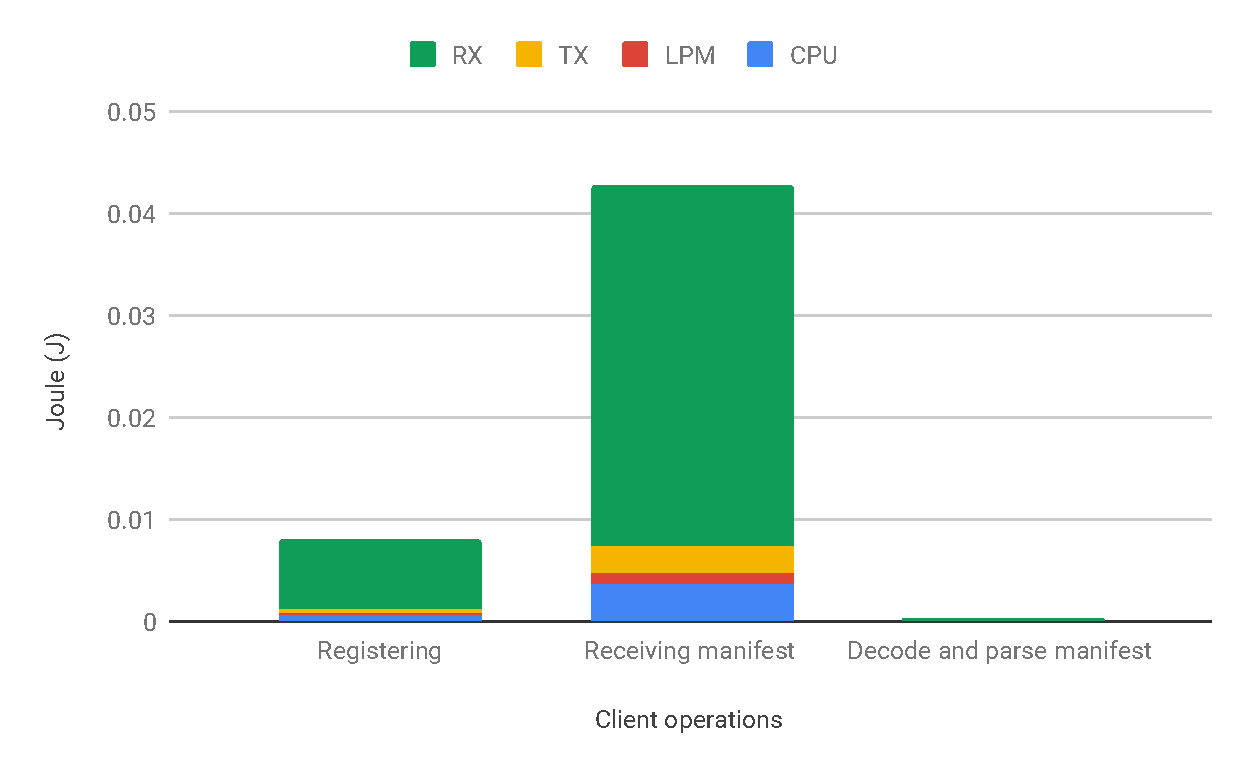
\includegraphics[scale=0.65]{images/client-operations-energy.pdf}
\end{figure}

\begin{figure}[h!]
    \caption{Average energy consumption for server operations.}
    \label{fig:server-operations-energy}
    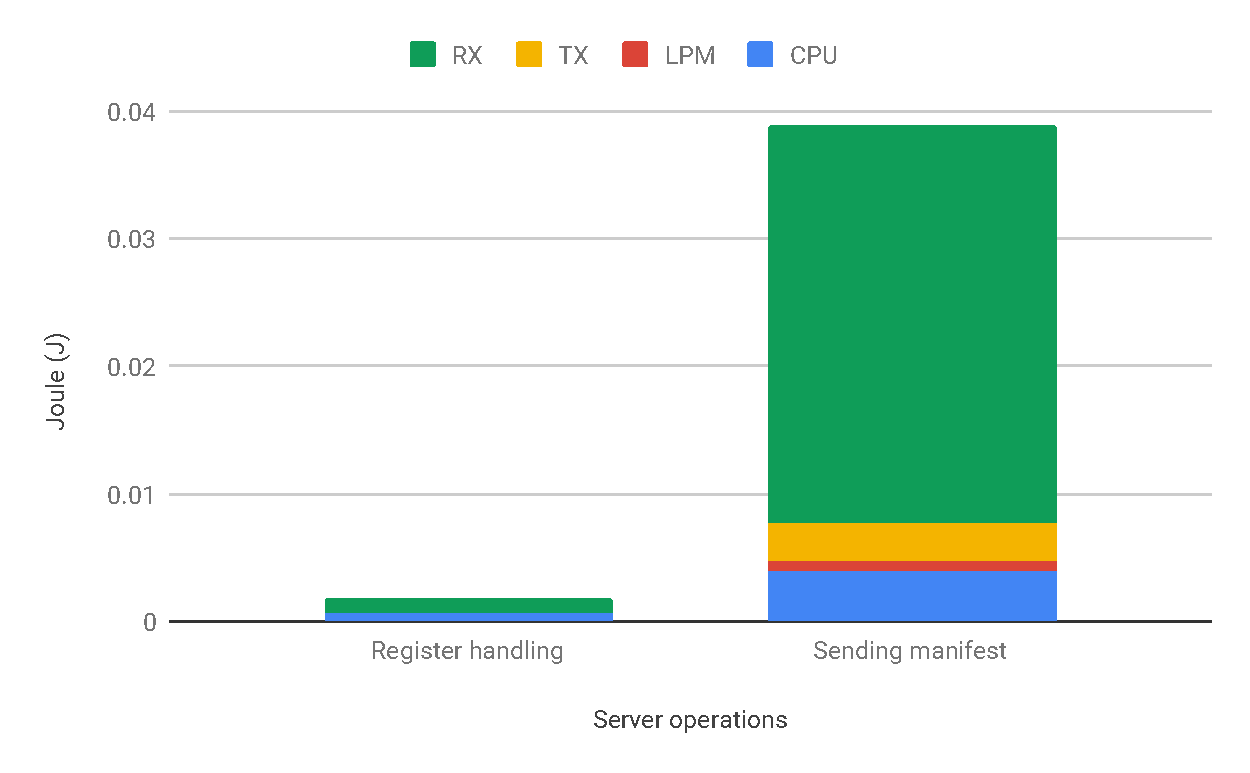
\includegraphics[scale=0.65]{images/server-operations-energy.pdf}
\end{figure}

\begin{figure}[h!]
    \caption{Average energy consumption for client during image transfer.}
    \label{fig:client-image-energy}
    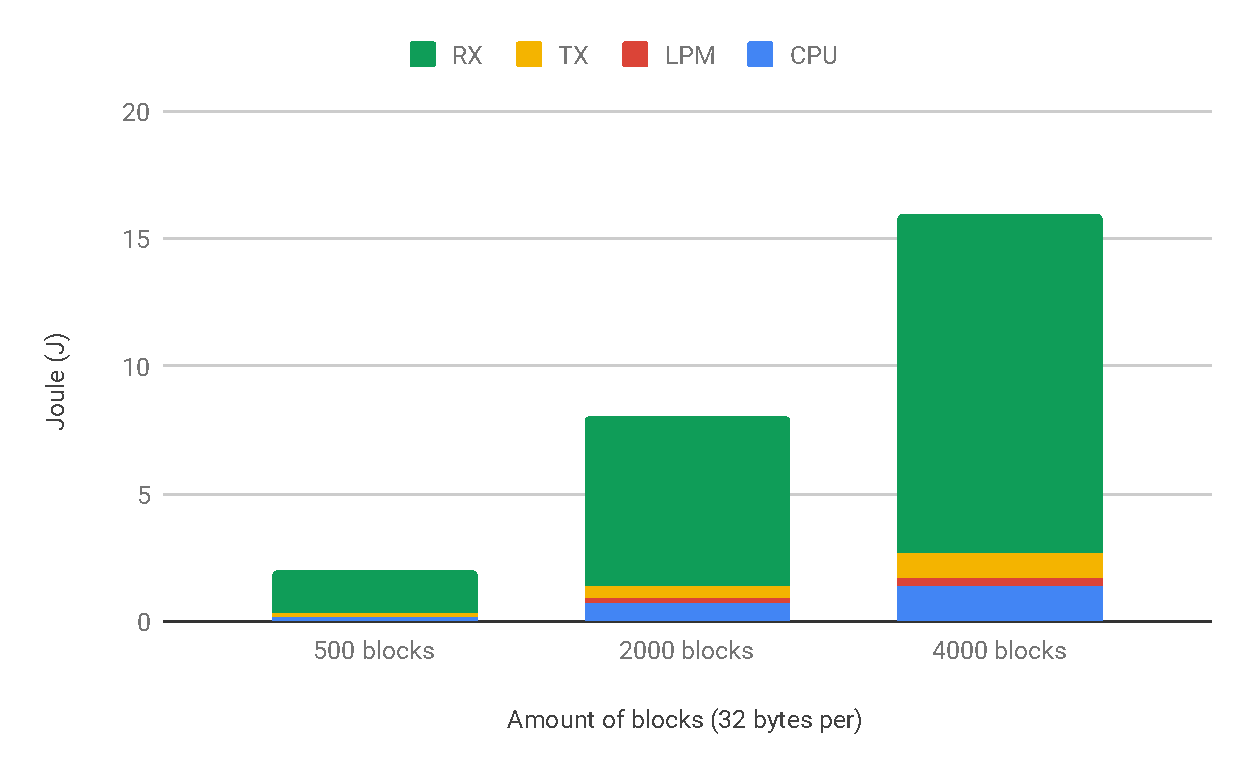
\includegraphics[scale=0.65]{images/client-image-energy.pdf}
\end{figure}

\begin{figure}[h!]
    \caption{Average energy consumption for server during image transfer.}
    \label{fig:server-image-energy}
    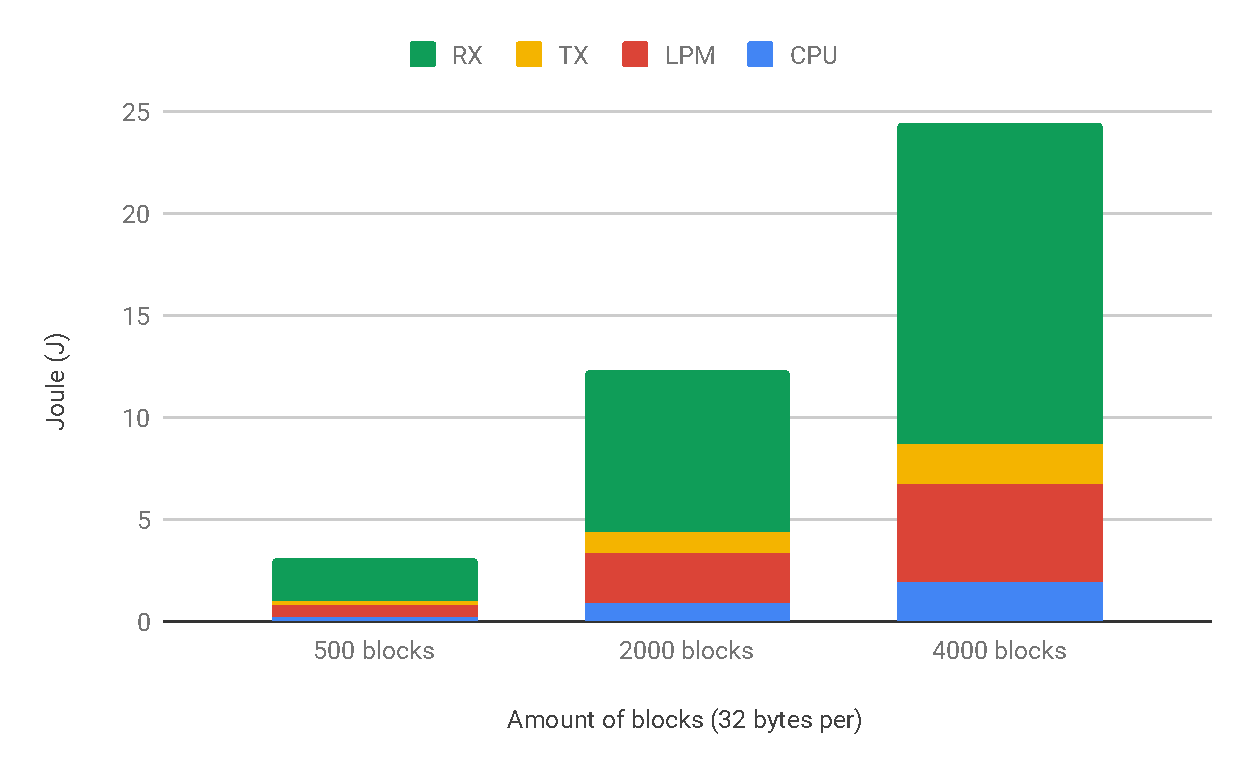
\includegraphics[scale=0.65]{images/server-image-energy.pdf}
\end{figure}

% Force new page so previous graphs appear in order
\newpage
\subsection{Communication Overhead}
\label{ssec:communication-overhead}
As discussed in Section~\ref{ssec:prototype-implementation}, some overhead is introduced
at the application layer as a consequence of using COSE encrypt. Each CoAP block sent by
the server during image transfer contains 32 bytes of data of which 8 is a tag used to
validate the ciphertext. Figure~\ref{fig:communication-overhead} shows this disparity.

\begin{figure}[h!]
    \caption{Bytes transferred vs actual data sent measured in bytes at the application layer.}
    \label{fig:communication-overhead}
    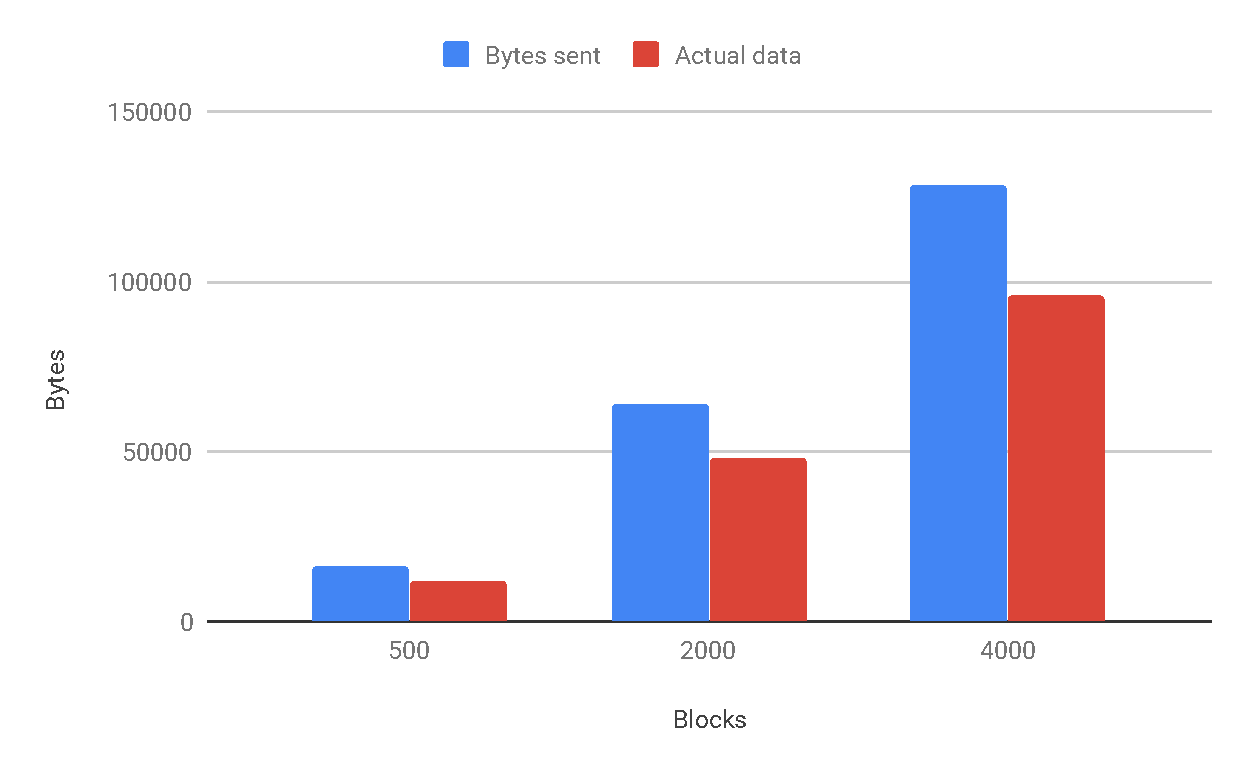
\includegraphics[scale=0.65]{images/communication-overhead.pdf}
\end{figure}

\subsection{Code Size}
\label{ssec:code-size}
When measuring code size the code was compiled with all debug macros set to 0, the
energest measurements removed, and no other Contiki-NG modules included except CoAP. As a
point of reference, a bare-bones example was also created. The bare-bones example only
contains the necessary imports to Contiki-NG and its CoAP engine and declares a process
with no code in it. It is the smallest runnable example for Firefly devices using the same
project configuration as the other source files. Its source code is found in
Appendix~\ref{app:bare-bones}. By running the tool \texttt{arm-none-eabi-size} on the
ELF-files the code size can be obtained, which is shown in Table~\ref{tab:code-size}.

\begin{table}[h!]
\begin{tabular}{l c r r r l}
text	&  data	 &  bss	 &  dec	 &  hex&filename\\
69982	&  1772	 &11303	 &83057	 &14472&bare-bones.elf\\
75956	&  1788	 &13599	 &91343	 &164cf&update-client.elf\\
77924	&  1884	 &11835	 &91643	 &165fb&update-server.elf
\end{tabular}
\caption{Code size for client and server prototypes.}
\label{tab:code-size}
\end{table}

\end{document}